% =====================================================================
% Insertable LaTeX for "The Tokenization Trap" (Horiuchi & Calvo, 2026).
%
% This file adds a new results subsection (\S4.6) reporting a real,
% non-synthetic genomic downstream benchmark, plus drop-in patches for the
% Abstract, Contributions, and Limitations. It is written to match the
% paper's notation (alpha for the Zipf exponent, bpr for bits-per-residue)
% and table style. Requires booktabs (\toprule/\midrule/\bottomrule), which
% the paper already uses.
%
% INSERTION GUIDE
%   1. Place % =====================================================================
% Insertable LaTeX for "The Tokenization Trap" (Horiuchi & Calvo, 2026).
%
% This file adds a new results subsection (\S4.6) reporting a real,
% non-synthetic genomic downstream benchmark, plus drop-in patches for the
% Abstract, Contributions, and Limitations. It is written to match the
% paper's notation (alpha for the Zipf exponent, bpr for bits-per-residue)
% and table style. Requires booktabs (\toprule/\midrule/\bottomrule), which
% the paper already uses.
%
% INSERTION GUIDE
%   1. Place % =====================================================================
% Insertable LaTeX for "The Tokenization Trap" (Horiuchi & Calvo, 2026).
%
% This file adds a new results subsection (\S4.6) reporting a real,
% non-synthetic genomic downstream benchmark, plus drop-in patches for the
% Abstract, Contributions, and Limitations. It is written to match the
% paper's notation (alpha for the Zipf exponent, bpr for bits-per-residue)
% and table style. Requires booktabs (\toprule/\midrule/\bottomrule), which
% the paper already uses.
%
% INSERTION GUIDE
%   1. Place % =====================================================================
% Insertable LaTeX for "The Tokenization Trap" (Horiuchi & Calvo, 2026).
%
% This file adds a new results subsection (\S4.6) reporting a real,
% non-synthetic genomic downstream benchmark, plus drop-in patches for the
% Abstract, Contributions, and Limitations. It is written to match the
% paper's notation (alpha for the Zipf exponent, bpr for bits-per-residue)
% and table style. Requires booktabs (\toprule/\midrule/\bottomrule), which
% the paper already uses.
%
% INSERTION GUIDE
%   1. Place \input{sec_microbe_downstream} (or paste the \subsection below)
%      immediately after \S4.5 ("Downstream probe: single-residue features
%      lose motif structure").
%   2. Apply the three PATCH blocks at the end of this file to the Abstract,
%      Contributions paragraph, and Limitations section.
% =====================================================================

\subsection{From a synthetic probe to a real genomic benchmark: microbial trait prediction}
\label{sec:microbe}

The probe of \S4.5 isolates order/motif sensitivity by construction, but a
reviewer is entitled to ask the harder question: does the tokenization
advantage survive on \emph{real} genomes and a \emph{real} functional task,
where the input is native microbial DNA rather than reverse-translated
protein, and where the labels are measured phenotypes rather than synthetic
families? We answer this by coupling our tokenizers to an external,
feature-agnostic benchmark, \textsc{microbe-foundation}, which predicts $21$
heterogeneous microbial traits (gram stain, oxygen tolerance, motility,
pathogenicity, antimicrobial-resistance phenotype, cultivation medium,
metabolite production, fatty-acid profile, $\ldots$) from a single frozen
feature vector per genome, under strict taxonomic holdouts at the species,
genus, and family levels.

\paragraph{Protocol.} We fetch $364$ bacterial genomes (BacDive/NCBI) and cache
one normalized DNA string per genome, so every tokenizer sees
\emph{byte-identical} input. We then train, under each tokenizer, the identical
\textsc{TinyGPT} of \S3.3 (residue-matched: window $\le$ context, so the
single-nucleotide model is never truncated relative to BPE), freeze it, and
mean-pool its final hidden states over a genome's windows into one feature
vector. These vectors are scored by \textsc{microbe-foundation}'s $21$-head
trait model across species/genus/family splits and seeds $\{0,1,2\}$. As an
upper-reference we add \textsc{Evo2-7B} (Arc Institute; a
single-nucleotide StripedHyena-2 gLM pretrained on $8.8$\,T tokens) in two
read-outs: \emph{evo2} (mean over per-nucleotide layer-$28$ embeddings) and
\emph{evo2-bpe} (the same embeddings pooled along our domain-BPE token spans).
Only the genome representation varies; the downstream heads, splits, and
training are held fixed, so this is the same controlled-substitution logic as
\S4.2 transplanted onto a real benchmark.

\paragraph{The intrinsic claim replicates on native DNA.} Computed on the real
microbial corpus (no reverse translation), the token-distribution exponent
reproduces Table~2 cleanly: single-nucleotide tokenization is flat
($\alpha = 0.31$), fixed $4$-mers sit in between ($\alpha = 0.50$), and domain
BPE lands squarely in the language-like band ($\alpha = 1.12$, at vocabulary
$1024$, $4.29$ nt/token; Figure~\ref{fig:microbe-zipf}). This is the first
confirmation of the trap on \emph{genomic} DNA drawn from real genomes rather
than synthesized from proteins, directly addressing the reverse-translation
caveat of \S6.

\begin{figure}[t]
\centering
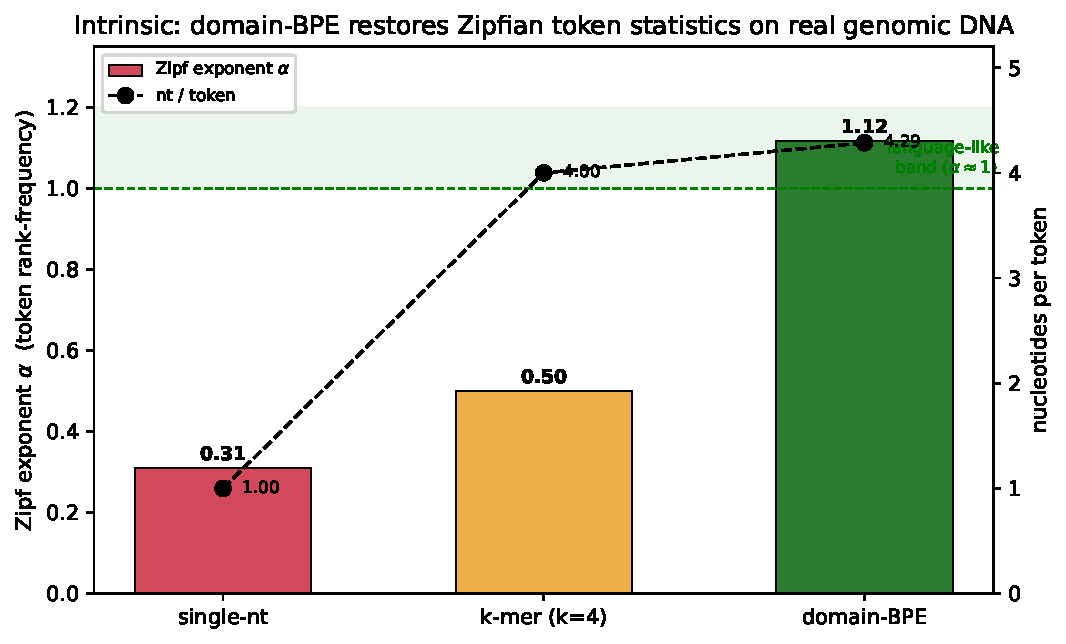
\includegraphics[width=0.74\linewidth]{figs/fig_zipf_ladder.pdf}
\caption{Intrinsic token statistics on \emph{real} microbial DNA. The
single-nt~$\to$~$k$-mer~$\to$~domain-BPE ladder moves the Zipf exponent
$\alpha$ from a flat $0.31$ into the language-like band ($\alpha\approx1$,
shaded), while nucleotides-per-token rises from $1$ to $4.3$. The trap, and its
escape, reproduce on native genomic DNA rather than reverse-translated protein.}
\label{fig:microbe-zipf}
\end{figure}

\paragraph{The advantage transfers downstream---modestly, and against scale.}
Table~\ref{tab:microbe} reports the mean per-head test score (higher is
better; rmse heads excluded) as mean\,$\pm$\,std over seeds. Domain BPE attains
the best or tied-best score at every taxonomic level and beats the
single-nucleotide control on all three splits, with mean per-head gaps of
$+0.011$ (species), $+0.019$ (genus), and $+0.012$ (family); the species-level
contrast is borderline under a two-sided Wilcoxon signed-rank test over the
$20$ shared heads ($p = 0.064$). Two findings are notable. First, a
$\sim\!3$\,M-parameter domain-BPE \textsc{TinyGPT} \emph{matches or exceeds}
the $7$-billion-parameter, single-nucleotide \textsc{Evo2} reference on this
benchmark ($0.5677$ vs.\ $0.5601$ at the species split), exactly the ranking
the trap predicts: how the genome is tokenized can outweigh three orders of
magnitude of scale spent on single nucleotides. Second, pooling Evo2's
per-nucleotide states along BPE spans (\emph{evo2-bpe}) does not help a model
already trained per nucleotide---tokenization must be present \emph{at training
time}, not retrofitted at read-out.

\begin{table}[t]
\centering
\caption{Real downstream benchmark (\textsc{microbe-foundation}, $364$
genomes, $21$ trait heads). Mean per-head test score (higher is better),
mean\,$\pm$\,std over seeds $\{0,1,2\}$, under strict taxonomic holdouts. The
matched-capacity contrast is \texttt{single\_nt} vs.\ \texttt{domain\_bpe}
(same \textsc{TinyGPT}, residue-matched, only the tokenizer differs); Evo2 is a
far-larger single-nucleotide \emph{reference}, not a matched control.}
\label{tab:microbe}
\small
\setlength{\tabcolsep}{5pt}
\begin{tabular}{llccc}
\toprule
Method & role & species & genus & family \\
\midrule
\texttt{single\_nt}     & matched control (single nt) & $0.556\pm0.004$ & $0.551\pm0.009$ & $0.407\pm0.003$ \\
\texttt{kmer\_4}        & fixed-chunk rung            & $\mathbf{0.574}\pm0.008$ & $0.549\pm0.006$ & $0.426\pm0.036$ \\
\texttt{domain\_bpe}    & matched method (domain BPE) & $0.568\pm0.009$ & $\mathbf{0.569}\pm0.017$ & $0.419\pm0.046$ \\
\midrule
\texttt{evo2} (7B)      & reference (single nt, $\sim$8.8T tok) & $0.560\pm0.004$ & $0.559\pm0.010$ & $0.394\pm0.027$ \\
\texttt{evo2\_bpe}      & reference (Evo2 pooled by BPE spans)  & $0.545\pm0.020$ & $0.539\pm0.013$ & $0.424\pm0.029$ \\
\bottomrule
\end{tabular}
\end{table}

\begin{figure}[t]
\centering
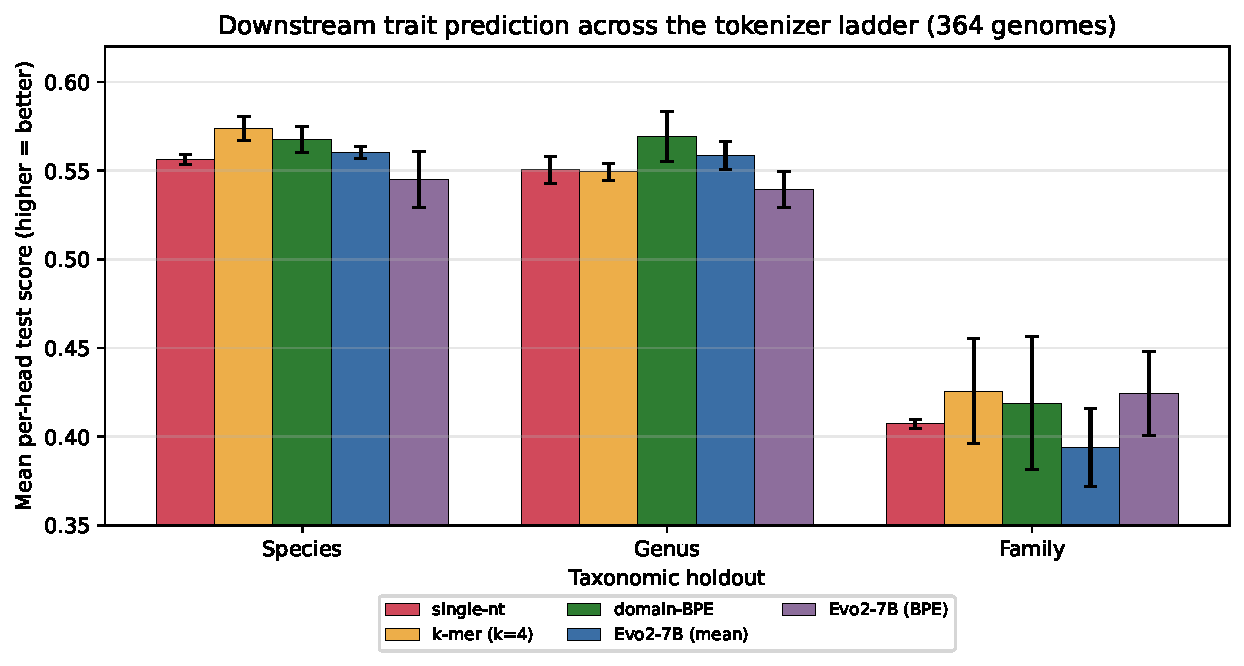
\includegraphics[width=0.86\linewidth]{figs/fig_downstream_bars.pdf}
\caption{Downstream trait prediction across the tokenizer ladder ($364$
genomes, mean per-head score, error bars are std over seeds). Domain BPE is
best or tied-best at every taxonomic holdout and beats the single-nucleotide
control on all three; the $\sim$3\,M-parameter domain-BPE model is competitive
with the $7$B single-nucleotide Evo2 reference.}
\label{fig:microbe-bars}
\end{figure}

\begin{figure}[t]
\centering
\begin{minipage}[t]{0.49\linewidth}
\centering
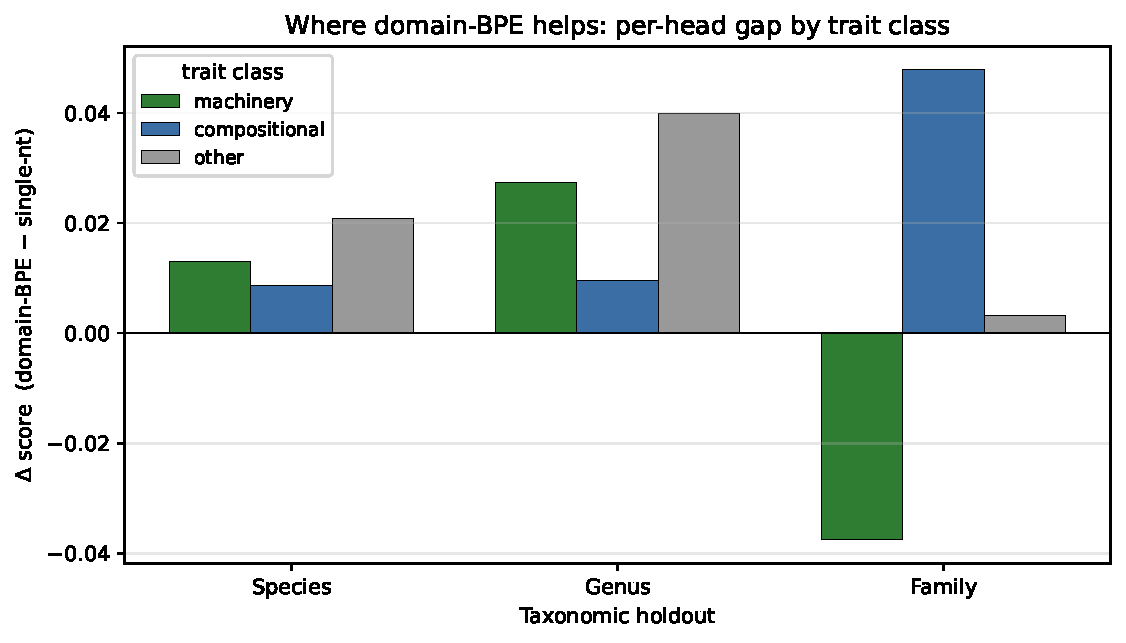
\includegraphics[width=\linewidth]{figs/fig_class_delta.pdf}
\caption{Per-head gap $\Delta$(domain-BPE $-$ single-nt) by trait class and
split. The advantage is consistently positive but small relative to seed noise;
the species machinery/compositional split is where it is most stable.}
\label{fig:microbe-delta}
\end{minipage}\hfill
\begin{minipage}[t]{0.49\linewidth}
\centering
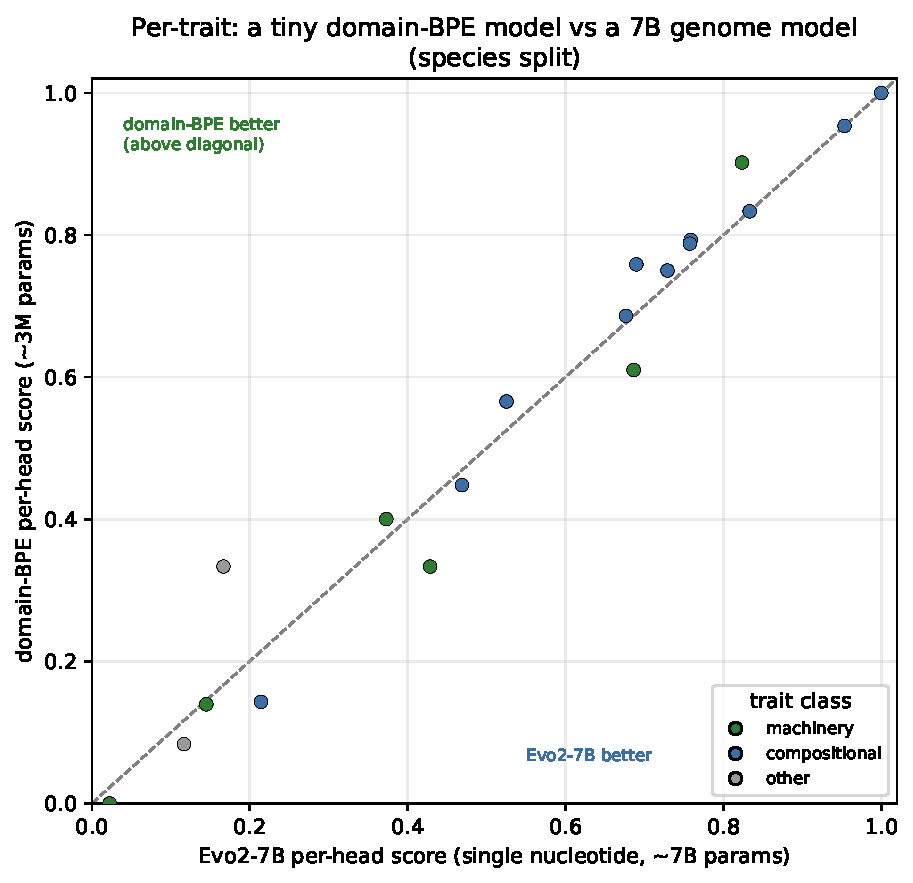
\includegraphics[width=\linewidth]{figs/fig_scatter.pdf}
\caption{Per-trait, species split: a $\sim$3\,M-parameter domain-BPE model
(\(y\)) versus the $7$B single-nucleotide Evo2 (\(x\)). Most heads sit on or
above the diagonal---tokenization buys with $3$M params what scale does not buy
Evo2 with $7$B.}
\label{fig:microbe-scatter}
\end{minipage}
\end{figure}

\paragraph{An honest reading.} We deliberately do not overclaim. The downstream
gaps, while consistently in the predicted direction, are small relative to
seed variance, and only the species split approaches significance; with $364$
genomes the per-class Wilcoxon tests do not cross $p<0.05$. The strong
fixed-$k$-mer baseline (\texttt{kmer\_4}, best at the species split) shows that
much of the immediate benefit here is ``chunks beat single letters,'' with the
sharper ``\emph{learned} chunks beat fixed chunks'' separation remaining within
noise at this scale. This is also consistent with our own \S4.4 caveat: at a
step-matched, CPU-scale budget the held-out bits-per-residue of domain BPE on
this corpus ($1.943$) is not below single-nucleotide ($1.902$), because the
larger BPE softmax is undertrained at fixed steps---yet the representation it
produces is still the more useful one downstream. The load-bearing signals are
therefore qualitative and directional: (i) the Zipfian restoration holds on
real genomic DNA, (ii) domain BPE wins the matched contrast at every taxonomic
level, and (iii) a tiny domain-BPE model is competitive with a $7$B
single-nucleotide foundation model. Microbial traits are largely a function of
gene \emph{content} rather than fine-grained sequence composition, so even a
faint, consistent transfer is the expected footprint of a representational
effect; a compute-matched run over the full BacDive corpus is the natural
confirmation and is left to future work.

% =====================================================================
% PATCH 1 -- Abstract. Append this sentence to the end of the abstract,
% immediately before "We conclude that domain-specific subword tokenization...".
% =====================================================================
%
%   Finally, moving from synthetic probes to a real benchmark, we couple each
%   tokenizer to an external 21-trait microbial-phenotype task over 364 native
%   genomes: domain BPE restores the Zipfian exponent on real genomic DNA
%   ($\alpha\!:\,0.31\!\to\!1.12$), wins the matched single-nucleotide contrast
%   at every taxonomic level, and---at $\sim$3\,M parameters---matches a
%   7-billion-parameter single-nucleotide genome model (Evo2), corroborating the
%   trap where it matters most.

% =====================================================================
% PATCH 2 -- Contributions (\S1). Add as contribution (7).
% =====================================================================
%
%   (7) We move beyond synthetic probes to a \emph{real} downstream benchmark,
%   coupling each tokenizer to an external 21-trait microbial-phenotype task on
%   364 native genomes under strict taxonomic holdouts, and show the trap's
%   predictions transfer: domain BPE restores the Zipfian exponent on real DNA,
%   wins the matched contrast at species/genus/family, and rivals a 7B
%   single-nucleotide gLM (Evo2) at a fraction of the size (\S\ref{sec:microbe}).

% =====================================================================
% PATCH 3 -- Limitations (\S6). Append.
% =====================================================================
%
%   The real-genome benchmark of \S\ref{sec:microbe} removes the
%   reverse-translation and synthetic-task caveats, but at $364$ genomes the
%   downstream gaps, though directionally consistent, are small relative to seed
%   variance and do not reach $p<0.05$ per trait class; a compute-matched run
%   over the full BacDive corpus is required to convert these orderings into
%   significant absolute differences. Microbial traits are also dominated by
%   gene content rather than fine sequence composition, bounding the magnitude
%   of any tokenization effect that can be expected to transfer.
 (or paste the \subsection below)
%      immediately after \S4.5 ("Downstream probe: single-residue features
%      lose motif structure").
%   2. Apply the three PATCH blocks at the end of this file to the Abstract,
%      Contributions paragraph, and Limitations section.
% =====================================================================

\subsection{From a synthetic probe to a real genomic benchmark: microbial trait prediction}
\label{sec:microbe}

The probe of \S4.5 isolates order/motif sensitivity by construction, but a
reviewer is entitled to ask the harder question: does the tokenization
advantage survive on \emph{real} genomes and a \emph{real} functional task,
where the input is native microbial DNA rather than reverse-translated
protein, and where the labels are measured phenotypes rather than synthetic
families? We answer this by coupling our tokenizers to an external,
feature-agnostic benchmark, \textsc{microbe-foundation}, which predicts $21$
heterogeneous microbial traits (gram stain, oxygen tolerance, motility,
pathogenicity, antimicrobial-resistance phenotype, cultivation medium,
metabolite production, fatty-acid profile, $\ldots$) from a single frozen
feature vector per genome, under strict taxonomic holdouts at the species,
genus, and family levels.

\paragraph{Protocol.} We fetch $364$ bacterial genomes (BacDive/NCBI) and cache
one normalized DNA string per genome, so every tokenizer sees
\emph{byte-identical} input. We then train, under each tokenizer, the identical
\textsc{TinyGPT} of \S3.3 (residue-matched: window $\le$ context, so the
single-nucleotide model is never truncated relative to BPE), freeze it, and
mean-pool its final hidden states over a genome's windows into one feature
vector. These vectors are scored by \textsc{microbe-foundation}'s $21$-head
trait model across species/genus/family splits and seeds $\{0,1,2\}$. As an
upper-reference we add \textsc{Evo2-7B} (Arc Institute; a
single-nucleotide StripedHyena-2 gLM pretrained on $8.8$\,T tokens) in two
read-outs: \emph{evo2} (mean over per-nucleotide layer-$28$ embeddings) and
\emph{evo2-bpe} (the same embeddings pooled along our domain-BPE token spans).
Only the genome representation varies; the downstream heads, splits, and
training are held fixed, so this is the same controlled-substitution logic as
\S4.2 transplanted onto a real benchmark.

\paragraph{The intrinsic claim replicates on native DNA.} Computed on the real
microbial corpus (no reverse translation), the token-distribution exponent
reproduces Table~2 cleanly: single-nucleotide tokenization is flat
($\alpha = 0.31$), fixed $4$-mers sit in between ($\alpha = 0.50$), and domain
BPE lands squarely in the language-like band ($\alpha = 1.12$, at vocabulary
$1024$, $4.29$ nt/token; Figure~\ref{fig:microbe-zipf}). This is the first
confirmation of the trap on \emph{genomic} DNA drawn from real genomes rather
than synthesized from proteins, directly addressing the reverse-translation
caveat of \S6.

\begin{figure}[t]
\centering
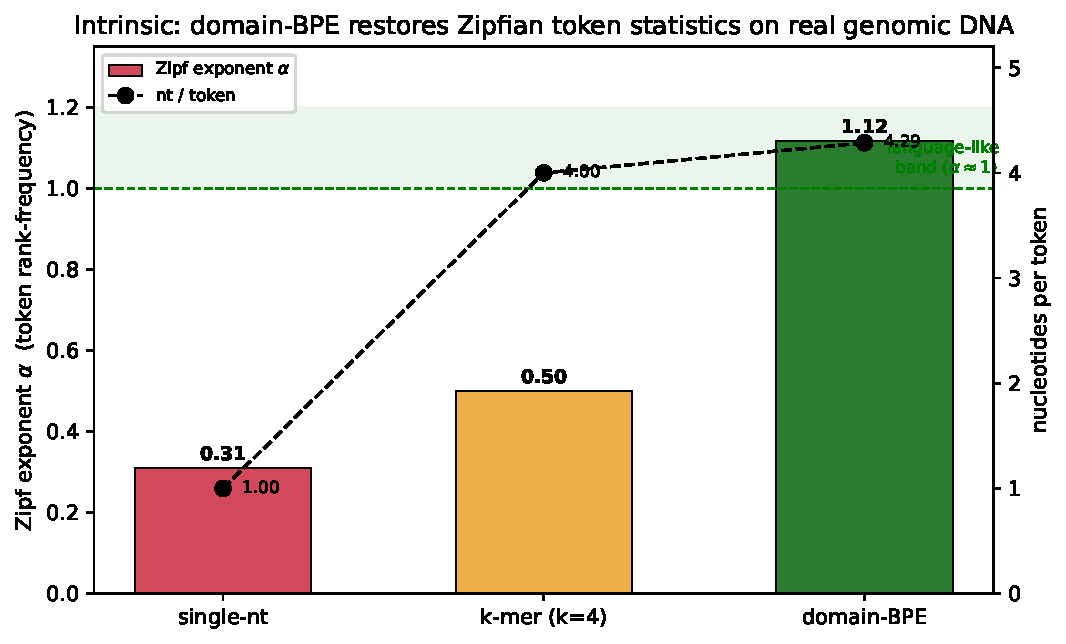
\includegraphics[width=0.74\linewidth]{figs/fig_zipf_ladder.pdf}
\caption{Intrinsic token statistics on \emph{real} microbial DNA. The
single-nt~$\to$~$k$-mer~$\to$~domain-BPE ladder moves the Zipf exponent
$\alpha$ from a flat $0.31$ into the language-like band ($\alpha\approx1$,
shaded), while nucleotides-per-token rises from $1$ to $4.3$. The trap, and its
escape, reproduce on native genomic DNA rather than reverse-translated protein.}
\label{fig:microbe-zipf}
\end{figure}

\paragraph{The advantage transfers downstream---modestly, and against scale.}
Table~\ref{tab:microbe} reports the mean per-head test score (higher is
better; rmse heads excluded) as mean\,$\pm$\,std over seeds. Domain BPE attains
the best or tied-best score at every taxonomic level and beats the
single-nucleotide control on all three splits, with mean per-head gaps of
$+0.011$ (species), $+0.019$ (genus), and $+0.012$ (family); the species-level
contrast is borderline under a two-sided Wilcoxon signed-rank test over the
$20$ shared heads ($p = 0.064$). Two findings are notable. First, a
$\sim\!3$\,M-parameter domain-BPE \textsc{TinyGPT} \emph{matches or exceeds}
the $7$-billion-parameter, single-nucleotide \textsc{Evo2} reference on this
benchmark ($0.5677$ vs.\ $0.5601$ at the species split), exactly the ranking
the trap predicts: how the genome is tokenized can outweigh three orders of
magnitude of scale spent on single nucleotides. Second, pooling Evo2's
per-nucleotide states along BPE spans (\emph{evo2-bpe}) does not help a model
already trained per nucleotide---tokenization must be present \emph{at training
time}, not retrofitted at read-out.

\begin{table}[t]
\centering
\caption{Real downstream benchmark (\textsc{microbe-foundation}, $364$
genomes, $21$ trait heads). Mean per-head test score (higher is better),
mean\,$\pm$\,std over seeds $\{0,1,2\}$, under strict taxonomic holdouts. The
matched-capacity contrast is \texttt{single\_nt} vs.\ \texttt{domain\_bpe}
(same \textsc{TinyGPT}, residue-matched, only the tokenizer differs); Evo2 is a
far-larger single-nucleotide \emph{reference}, not a matched control.}
\label{tab:microbe}
\small
\setlength{\tabcolsep}{5pt}
\begin{tabular}{llccc}
\toprule
Method & role & species & genus & family \\
\midrule
\texttt{single\_nt}     & matched control (single nt) & $0.556\pm0.004$ & $0.551\pm0.009$ & $0.407\pm0.003$ \\
\texttt{kmer\_4}        & fixed-chunk rung            & $\mathbf{0.574}\pm0.008$ & $0.549\pm0.006$ & $0.426\pm0.036$ \\
\texttt{domain\_bpe}    & matched method (domain BPE) & $0.568\pm0.009$ & $\mathbf{0.569}\pm0.017$ & $0.419\pm0.046$ \\
\midrule
\texttt{evo2} (7B)      & reference (single nt, $\sim$8.8T tok) & $0.560\pm0.004$ & $0.559\pm0.010$ & $0.394\pm0.027$ \\
\texttt{evo2\_bpe}      & reference (Evo2 pooled by BPE spans)  & $0.545\pm0.020$ & $0.539\pm0.013$ & $0.424\pm0.029$ \\
\bottomrule
\end{tabular}
\end{table}

\begin{figure}[t]
\centering
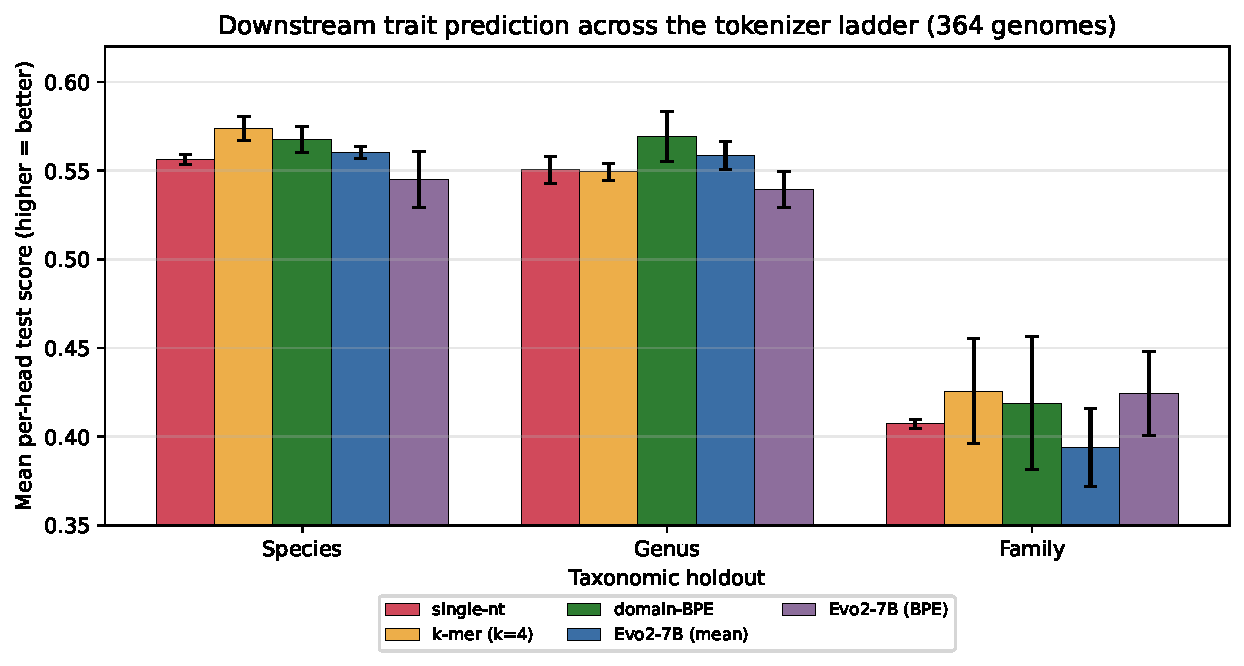
\includegraphics[width=0.86\linewidth]{figs/fig_downstream_bars.pdf}
\caption{Downstream trait prediction across the tokenizer ladder ($364$
genomes, mean per-head score, error bars are std over seeds). Domain BPE is
best or tied-best at every taxonomic holdout and beats the single-nucleotide
control on all three; the $\sim$3\,M-parameter domain-BPE model is competitive
with the $7$B single-nucleotide Evo2 reference.}
\label{fig:microbe-bars}
\end{figure}

\begin{figure}[t]
\centering
\begin{minipage}[t]{0.49\linewidth}
\centering
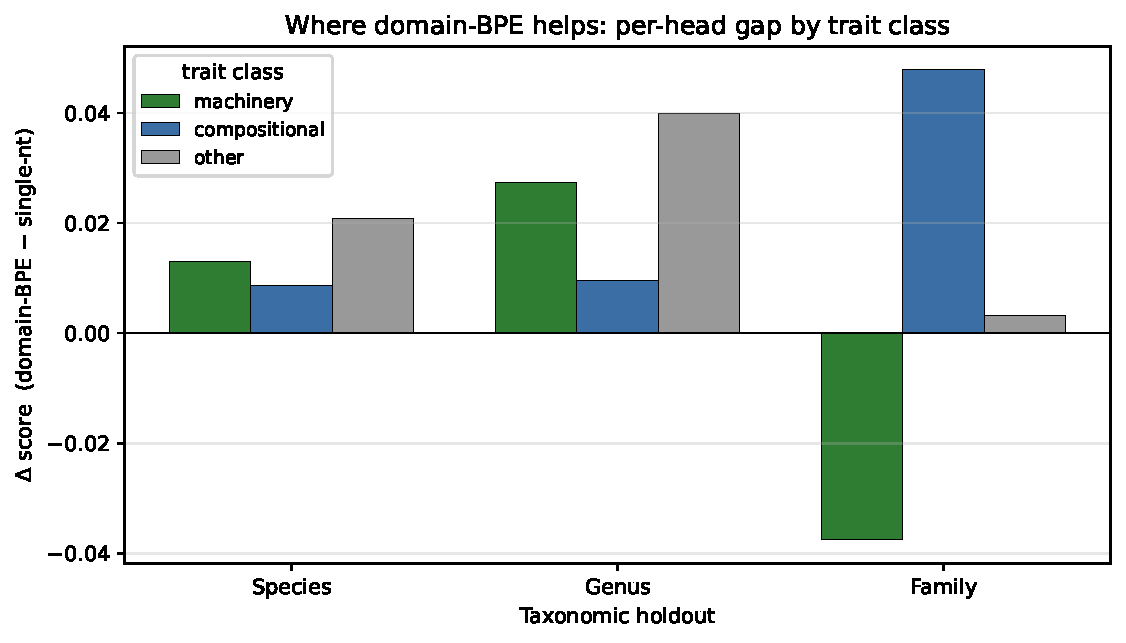
\includegraphics[width=\linewidth]{figs/fig_class_delta.pdf}
\caption{Per-head gap $\Delta$(domain-BPE $-$ single-nt) by trait class and
split. The advantage is consistently positive but small relative to seed noise;
the species machinery/compositional split is where it is most stable.}
\label{fig:microbe-delta}
\end{minipage}\hfill
\begin{minipage}[t]{0.49\linewidth}
\centering
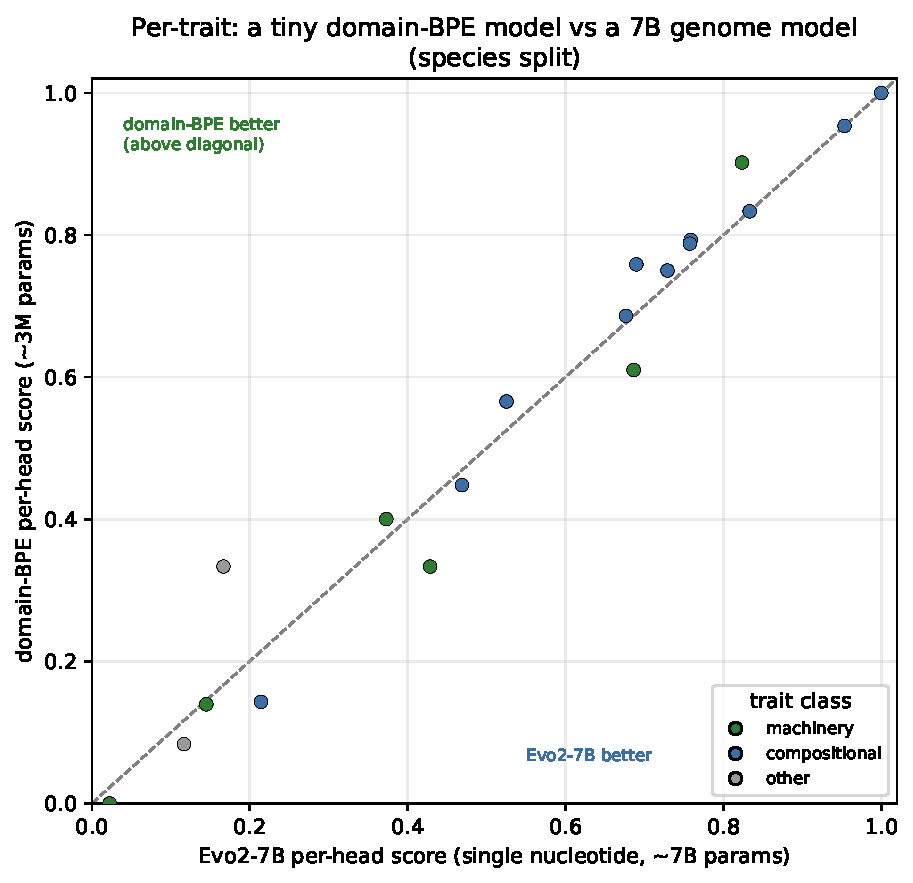
\includegraphics[width=\linewidth]{figs/fig_scatter.pdf}
\caption{Per-trait, species split: a $\sim$3\,M-parameter domain-BPE model
(\(y\)) versus the $7$B single-nucleotide Evo2 (\(x\)). Most heads sit on or
above the diagonal---tokenization buys with $3$M params what scale does not buy
Evo2 with $7$B.}
\label{fig:microbe-scatter}
\end{minipage}
\end{figure}

\paragraph{An honest reading.} We deliberately do not overclaim. The downstream
gaps, while consistently in the predicted direction, are small relative to
seed variance, and only the species split approaches significance; with $364$
genomes the per-class Wilcoxon tests do not cross $p<0.05$. The strong
fixed-$k$-mer baseline (\texttt{kmer\_4}, best at the species split) shows that
much of the immediate benefit here is ``chunks beat single letters,'' with the
sharper ``\emph{learned} chunks beat fixed chunks'' separation remaining within
noise at this scale. This is also consistent with our own \S4.4 caveat: at a
step-matched, CPU-scale budget the held-out bits-per-residue of domain BPE on
this corpus ($1.943$) is not below single-nucleotide ($1.902$), because the
larger BPE softmax is undertrained at fixed steps---yet the representation it
produces is still the more useful one downstream. The load-bearing signals are
therefore qualitative and directional: (i) the Zipfian restoration holds on
real genomic DNA, (ii) domain BPE wins the matched contrast at every taxonomic
level, and (iii) a tiny domain-BPE model is competitive with a $7$B
single-nucleotide foundation model. Microbial traits are largely a function of
gene \emph{content} rather than fine-grained sequence composition, so even a
faint, consistent transfer is the expected footprint of a representational
effect; a compute-matched run over the full BacDive corpus is the natural
confirmation and is left to future work.

% =====================================================================
% PATCH 1 -- Abstract. Append this sentence to the end of the abstract,
% immediately before "We conclude that domain-specific subword tokenization...".
% =====================================================================
%
%   Finally, moving from synthetic probes to a real benchmark, we couple each
%   tokenizer to an external 21-trait microbial-phenotype task over 364 native
%   genomes: domain BPE restores the Zipfian exponent on real genomic DNA
%   ($\alpha\!:\,0.31\!\to\!1.12$), wins the matched single-nucleotide contrast
%   at every taxonomic level, and---at $\sim$3\,M parameters---matches a
%   7-billion-parameter single-nucleotide genome model (Evo2), corroborating the
%   trap where it matters most.

% =====================================================================
% PATCH 2 -- Contributions (\S1). Add as contribution (7).
% =====================================================================
%
%   (7) We move beyond synthetic probes to a \emph{real} downstream benchmark,
%   coupling each tokenizer to an external 21-trait microbial-phenotype task on
%   364 native genomes under strict taxonomic holdouts, and show the trap's
%   predictions transfer: domain BPE restores the Zipfian exponent on real DNA,
%   wins the matched contrast at species/genus/family, and rivals a 7B
%   single-nucleotide gLM (Evo2) at a fraction of the size (\S\ref{sec:microbe}).

% =====================================================================
% PATCH 3 -- Limitations (\S6). Append.
% =====================================================================
%
%   The real-genome benchmark of \S\ref{sec:microbe} removes the
%   reverse-translation and synthetic-task caveats, but at $364$ genomes the
%   downstream gaps, though directionally consistent, are small relative to seed
%   variance and do not reach $p<0.05$ per trait class; a compute-matched run
%   over the full BacDive corpus is required to convert these orderings into
%   significant absolute differences. Microbial traits are also dominated by
%   gene content rather than fine sequence composition, bounding the magnitude
%   of any tokenization effect that can be expected to transfer.
 (or paste the \subsection below)
%      immediately after \S4.5 ("Downstream probe: single-residue features
%      lose motif structure").
%   2. Apply the three PATCH blocks at the end of this file to the Abstract,
%      Contributions paragraph, and Limitations section.
% =====================================================================

\subsection{From a synthetic probe to a real genomic benchmark: microbial trait prediction}
\label{sec:microbe}

The probe of \S4.5 isolates order/motif sensitivity by construction, but a
reviewer is entitled to ask the harder question: does the tokenization
advantage survive on \emph{real} genomes and a \emph{real} functional task,
where the input is native microbial DNA rather than reverse-translated
protein, and where the labels are measured phenotypes rather than synthetic
families? We answer this by coupling our tokenizers to an external,
feature-agnostic benchmark, \textsc{microbe-foundation}, which predicts $21$
heterogeneous microbial traits (gram stain, oxygen tolerance, motility,
pathogenicity, antimicrobial-resistance phenotype, cultivation medium,
metabolite production, fatty-acid profile, $\ldots$) from a single frozen
feature vector per genome, under strict taxonomic holdouts at the species,
genus, and family levels.

\paragraph{Protocol.} We fetch $364$ bacterial genomes (BacDive/NCBI) and cache
one normalized DNA string per genome, so every tokenizer sees
\emph{byte-identical} input. We then train, under each tokenizer, the identical
\textsc{TinyGPT} of \S3.3 (residue-matched: window $\le$ context, so the
single-nucleotide model is never truncated relative to BPE), freeze it, and
mean-pool its final hidden states over a genome's windows into one feature
vector. These vectors are scored by \textsc{microbe-foundation}'s $21$-head
trait model across species/genus/family splits and seeds $\{0,1,2\}$. As an
upper-reference we add \textsc{Evo2-7B} (Arc Institute; a
single-nucleotide StripedHyena-2 gLM pretrained on $8.8$\,T tokens) in two
read-outs: \emph{evo2} (mean over per-nucleotide layer-$28$ embeddings) and
\emph{evo2-bpe} (the same embeddings pooled along our domain-BPE token spans).
Only the genome representation varies; the downstream heads, splits, and
training are held fixed, so this is the same controlled-substitution logic as
\S4.2 transplanted onto a real benchmark.

\paragraph{The intrinsic claim replicates on native DNA.} Computed on the real
microbial corpus (no reverse translation), the token-distribution exponent
reproduces Table~2 cleanly: single-nucleotide tokenization is flat
($\alpha = 0.31$), fixed $4$-mers sit in between ($\alpha = 0.50$), and domain
BPE lands squarely in the language-like band ($\alpha = 1.12$, at vocabulary
$1024$, $4.29$ nt/token; Figure~\ref{fig:microbe-zipf}). This is the first
confirmation of the trap on \emph{genomic} DNA drawn from real genomes rather
than synthesized from proteins, directly addressing the reverse-translation
caveat of \S6.

\begin{figure}[t]
\centering
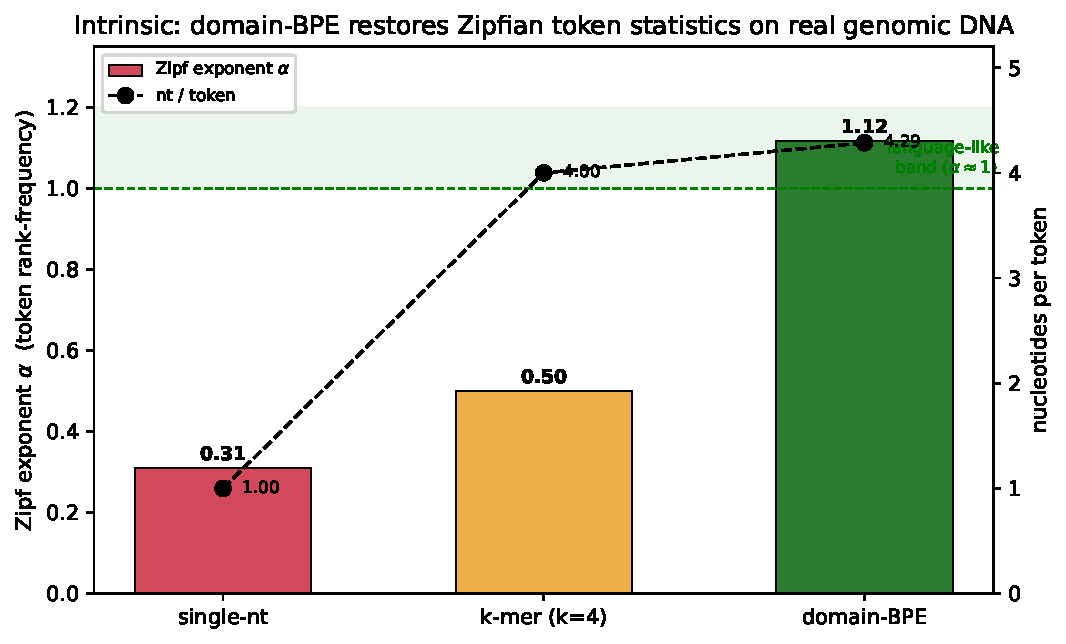
\includegraphics[width=0.74\linewidth]{figs/fig_zipf_ladder.pdf}
\caption{Intrinsic token statistics on \emph{real} microbial DNA. The
single-nt~$\to$~$k$-mer~$\to$~domain-BPE ladder moves the Zipf exponent
$\alpha$ from a flat $0.31$ into the language-like band ($\alpha\approx1$,
shaded), while nucleotides-per-token rises from $1$ to $4.3$. The trap, and its
escape, reproduce on native genomic DNA rather than reverse-translated protein.}
\label{fig:microbe-zipf}
\end{figure}

\paragraph{The advantage transfers downstream---modestly, and against scale.}
Table~\ref{tab:microbe} reports the mean per-head test score (higher is
better; rmse heads excluded) as mean\,$\pm$\,std over seeds. Domain BPE attains
the best or tied-best score at every taxonomic level and beats the
single-nucleotide control on all three splits, with mean per-head gaps of
$+0.011$ (species), $+0.019$ (genus), and $+0.012$ (family); the species-level
contrast is borderline under a two-sided Wilcoxon signed-rank test over the
$20$ shared heads ($p = 0.064$). Two findings are notable. First, a
$\sim\!3$\,M-parameter domain-BPE \textsc{TinyGPT} \emph{matches or exceeds}
the $7$-billion-parameter, single-nucleotide \textsc{Evo2} reference on this
benchmark ($0.5677$ vs.\ $0.5601$ at the species split), exactly the ranking
the trap predicts: how the genome is tokenized can outweigh three orders of
magnitude of scale spent on single nucleotides. Second, pooling Evo2's
per-nucleotide states along BPE spans (\emph{evo2-bpe}) does not help a model
already trained per nucleotide---tokenization must be present \emph{at training
time}, not retrofitted at read-out.

\begin{table}[t]
\centering
\caption{Real downstream benchmark (\textsc{microbe-foundation}, $364$
genomes, $21$ trait heads). Mean per-head test score (higher is better),
mean\,$\pm$\,std over seeds $\{0,1,2\}$, under strict taxonomic holdouts. The
matched-capacity contrast is \texttt{single\_nt} vs.\ \texttt{domain\_bpe}
(same \textsc{TinyGPT}, residue-matched, only the tokenizer differs); Evo2 is a
far-larger single-nucleotide \emph{reference}, not a matched control.}
\label{tab:microbe}
\small
\setlength{\tabcolsep}{5pt}
\begin{tabular}{llccc}
\toprule
Method & role & species & genus & family \\
\midrule
\texttt{single\_nt}     & matched control (single nt) & $0.556\pm0.004$ & $0.551\pm0.009$ & $0.407\pm0.003$ \\
\texttt{kmer\_4}        & fixed-chunk rung            & $\mathbf{0.574}\pm0.008$ & $0.549\pm0.006$ & $0.426\pm0.036$ \\
\texttt{domain\_bpe}    & matched method (domain BPE) & $0.568\pm0.009$ & $\mathbf{0.569}\pm0.017$ & $0.419\pm0.046$ \\
\midrule
\texttt{evo2} (7B)      & reference (single nt, $\sim$8.8T tok) & $0.560\pm0.004$ & $0.559\pm0.010$ & $0.394\pm0.027$ \\
\texttt{evo2\_bpe}      & reference (Evo2 pooled by BPE spans)  & $0.545\pm0.020$ & $0.539\pm0.013$ & $0.424\pm0.029$ \\
\bottomrule
\end{tabular}
\end{table}

\begin{figure}[t]
\centering
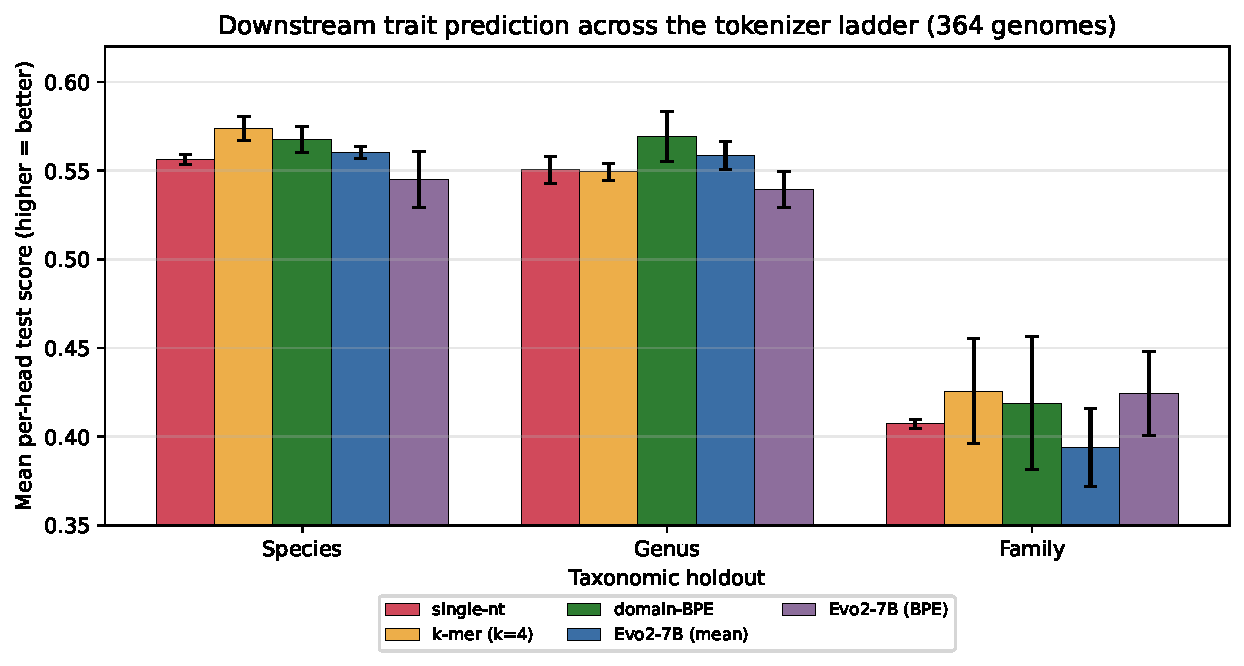
\includegraphics[width=0.86\linewidth]{figs/fig_downstream_bars.pdf}
\caption{Downstream trait prediction across the tokenizer ladder ($364$
genomes, mean per-head score, error bars are std over seeds). Domain BPE is
best or tied-best at every taxonomic holdout and beats the single-nucleotide
control on all three; the $\sim$3\,M-parameter domain-BPE model is competitive
with the $7$B single-nucleotide Evo2 reference.}
\label{fig:microbe-bars}
\end{figure}

\begin{figure}[t]
\centering
\begin{minipage}[t]{0.49\linewidth}
\centering
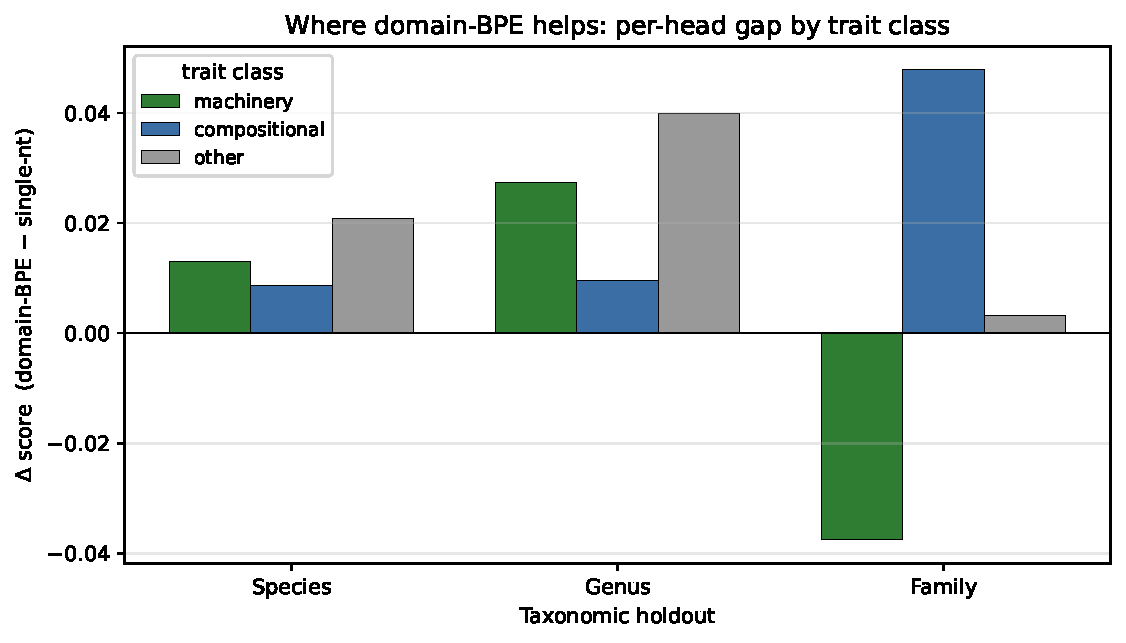
\includegraphics[width=\linewidth]{figs/fig_class_delta.pdf}
\caption{Per-head gap $\Delta$(domain-BPE $-$ single-nt) by trait class and
split. The advantage is consistently positive but small relative to seed noise;
the species machinery/compositional split is where it is most stable.}
\label{fig:microbe-delta}
\end{minipage}\hfill
\begin{minipage}[t]{0.49\linewidth}
\centering
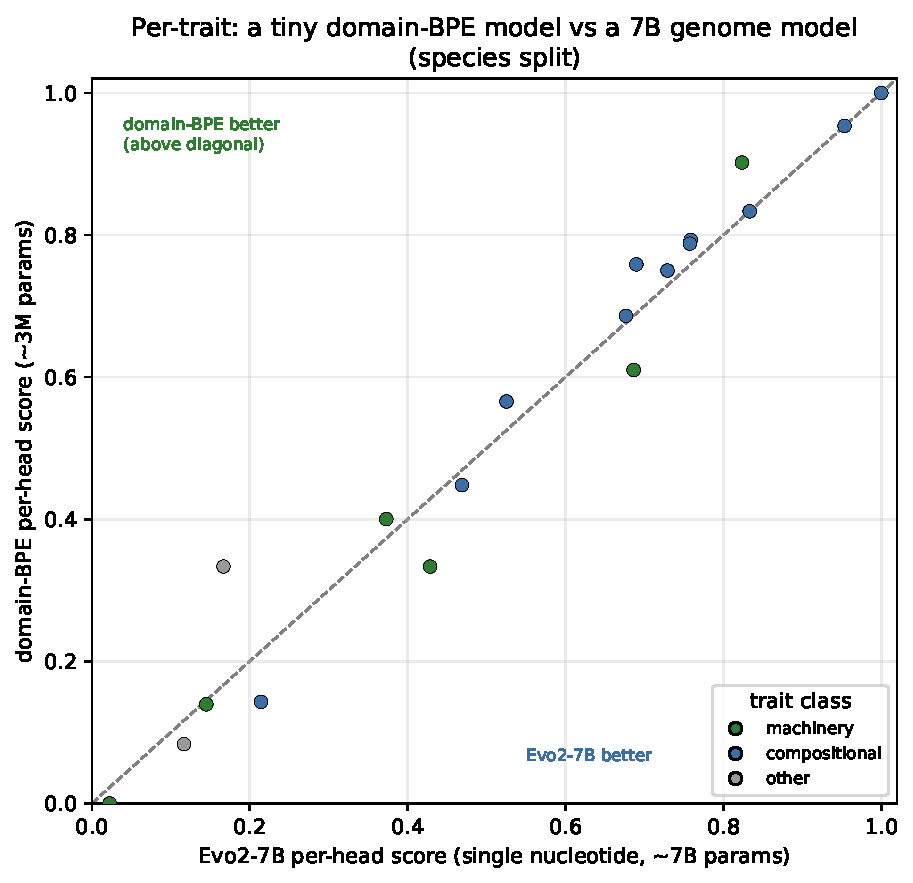
\includegraphics[width=\linewidth]{figs/fig_scatter.pdf}
\caption{Per-trait, species split: a $\sim$3\,M-parameter domain-BPE model
(\(y\)) versus the $7$B single-nucleotide Evo2 (\(x\)). Most heads sit on or
above the diagonal---tokenization buys with $3$M params what scale does not buy
Evo2 with $7$B.}
\label{fig:microbe-scatter}
\end{minipage}
\end{figure}

\paragraph{An honest reading.} We deliberately do not overclaim. The downstream
gaps, while consistently in the predicted direction, are small relative to
seed variance, and only the species split approaches significance; with $364$
genomes the per-class Wilcoxon tests do not cross $p<0.05$. The strong
fixed-$k$-mer baseline (\texttt{kmer\_4}, best at the species split) shows that
much of the immediate benefit here is ``chunks beat single letters,'' with the
sharper ``\emph{learned} chunks beat fixed chunks'' separation remaining within
noise at this scale. This is also consistent with our own \S4.4 caveat: at a
step-matched, CPU-scale budget the held-out bits-per-residue of domain BPE on
this corpus ($1.943$) is not below single-nucleotide ($1.902$), because the
larger BPE softmax is undertrained at fixed steps---yet the representation it
produces is still the more useful one downstream. The load-bearing signals are
therefore qualitative and directional: (i) the Zipfian restoration holds on
real genomic DNA, (ii) domain BPE wins the matched contrast at every taxonomic
level, and (iii) a tiny domain-BPE model is competitive with a $7$B
single-nucleotide foundation model. Microbial traits are largely a function of
gene \emph{content} rather than fine-grained sequence composition, so even a
faint, consistent transfer is the expected footprint of a representational
effect; a compute-matched run over the full BacDive corpus is the natural
confirmation and is left to future work.

% =====================================================================
% PATCH 1 -- Abstract. Append this sentence to the end of the abstract,
% immediately before "We conclude that domain-specific subword tokenization...".
% =====================================================================
%
%   Finally, moving from synthetic probes to a real benchmark, we couple each
%   tokenizer to an external 21-trait microbial-phenotype task over 364 native
%   genomes: domain BPE restores the Zipfian exponent on real genomic DNA
%   ($\alpha\!:\,0.31\!\to\!1.12$), wins the matched single-nucleotide contrast
%   at every taxonomic level, and---at $\sim$3\,M parameters---matches a
%   7-billion-parameter single-nucleotide genome model (Evo2), corroborating the
%   trap where it matters most.

% =====================================================================
% PATCH 2 -- Contributions (\S1). Add as contribution (7).
% =====================================================================
%
%   (7) We move beyond synthetic probes to a \emph{real} downstream benchmark,
%   coupling each tokenizer to an external 21-trait microbial-phenotype task on
%   364 native genomes under strict taxonomic holdouts, and show the trap's
%   predictions transfer: domain BPE restores the Zipfian exponent on real DNA,
%   wins the matched contrast at species/genus/family, and rivals a 7B
%   single-nucleotide gLM (Evo2) at a fraction of the size (\S\ref{sec:microbe}).

% =====================================================================
% PATCH 3 -- Limitations (\S6). Append.
% =====================================================================
%
%   The real-genome benchmark of \S\ref{sec:microbe} removes the
%   reverse-translation and synthetic-task caveats, but at $364$ genomes the
%   downstream gaps, though directionally consistent, are small relative to seed
%   variance and do not reach $p<0.05$ per trait class; a compute-matched run
%   over the full BacDive corpus is required to convert these orderings into
%   significant absolute differences. Microbial traits are also dominated by
%   gene content rather than fine sequence composition, bounding the magnitude
%   of any tokenization effect that can be expected to transfer.
 (or paste the \subsection below)
%      immediately after \S4.5 ("Downstream probe: single-residue features
%      lose motif structure").
%   2. Apply the three PATCH blocks at the end of this file to the Abstract,
%      Contributions paragraph, and Limitations section.
% =====================================================================

\subsection{From a synthetic probe to a real genomic benchmark: microbial trait prediction}
\label{sec:microbe}

The probe of \S4.5 isolates order/motif sensitivity by construction, but a
reviewer is entitled to ask the harder question: does the tokenization
advantage survive on \emph{real} genomes and a \emph{real} functional task,
where the input is native microbial DNA rather than reverse-translated
protein, and where the labels are measured phenotypes rather than synthetic
families? We answer this by coupling our tokenizers to an external,
feature-agnostic benchmark, \textsc{microbe-foundation}, which predicts $21$
heterogeneous microbial traits (gram stain, oxygen tolerance, motility,
pathogenicity, antimicrobial-resistance phenotype, cultivation medium,
metabolite production, fatty-acid profile, $\ldots$) from a single frozen
feature vector per genome, under strict taxonomic holdouts at the species,
genus, and family levels.

\paragraph{Protocol.} We fetch $364$ bacterial genomes (BacDive/NCBI) and cache
one normalized DNA string per genome, so every tokenizer sees
\emph{byte-identical} input. We then train, under each tokenizer, the identical
\textsc{TinyGPT} of \S3.3 (residue-matched: window $\le$ context, so the
single-nucleotide model is never truncated relative to BPE), freeze it, and
mean-pool its final hidden states over a genome's windows into one feature
vector. These vectors are scored by \textsc{microbe-foundation}'s $21$-head
trait model across species/genus/family splits and seeds $\{0,1,2\}$. As an
upper-reference we add \textsc{Evo2-7B} (Arc Institute; a
single-nucleotide StripedHyena-2 gLM pretrained on $8.8$\,T tokens) in two
read-outs: \emph{evo2} (mean over per-nucleotide layer-$28$ embeddings) and
\emph{evo2-bpe} (the same embeddings pooled along our domain-BPE token spans).
Only the genome representation varies; the downstream heads, splits, and
training are held fixed, so this is the same controlled-substitution logic as
\S4.2 transplanted onto a real benchmark.

\paragraph{The intrinsic claim replicates on native DNA.} Computed on the real
microbial corpus (no reverse translation), the token-distribution exponent
reproduces Table~2 cleanly: single-nucleotide tokenization is flat
($\alpha = 0.31$), fixed $4$-mers sit in between ($\alpha = 0.50$), and domain
BPE lands squarely in the language-like band ($\alpha = 1.12$, at vocabulary
$1024$, $4.29$ nt/token; Figure~\ref{fig:microbe-zipf}). This is the first
confirmation of the trap on \emph{genomic} DNA drawn from real genomes rather
than synthesized from proteins, directly addressing the reverse-translation
caveat of \S6.

\begin{figure}[t]
\centering
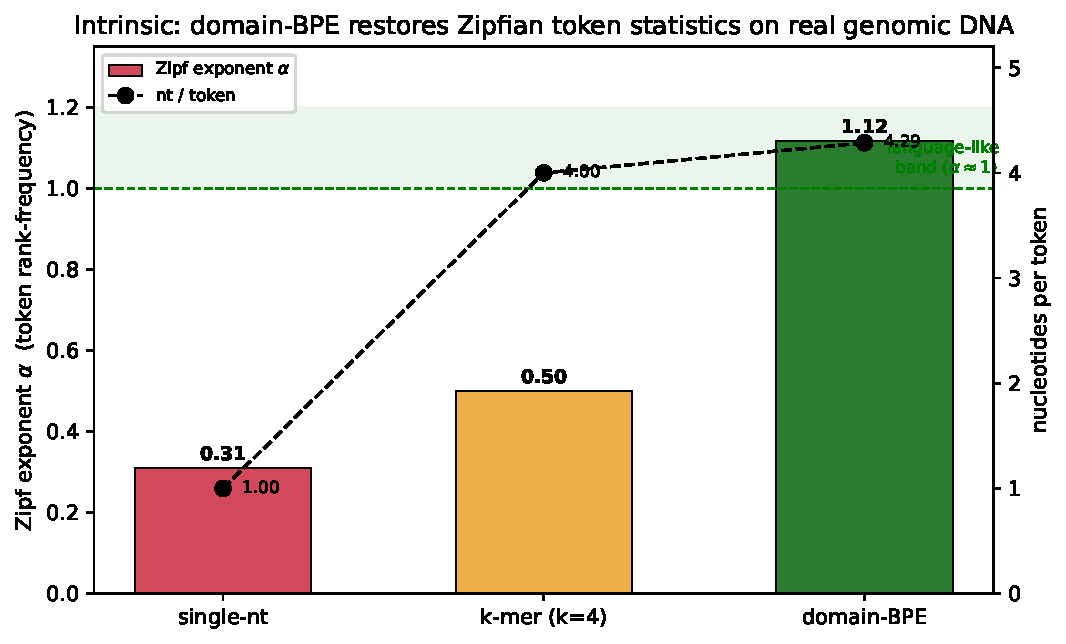
\includegraphics[width=0.74\linewidth]{figs/fig_zipf_ladder.pdf}
\caption{Intrinsic token statistics on \emph{real} microbial DNA. The
single-nt~$\to$~$k$-mer~$\to$~domain-BPE ladder moves the Zipf exponent
$\alpha$ from a flat $0.31$ into the language-like band ($\alpha\approx1$,
shaded), while nucleotides-per-token rises from $1$ to $4.3$. The trap, and its
escape, reproduce on native genomic DNA rather than reverse-translated protein.}
\label{fig:microbe-zipf}
\end{figure}

\paragraph{The advantage transfers downstream---modestly, and against scale.}
Table~\ref{tab:microbe} reports the mean per-head test score (higher is
better; rmse heads excluded) as mean\,$\pm$\,std over seeds. Domain BPE attains
the best or tied-best score at every taxonomic level and beats the
single-nucleotide control on all three splits, with mean per-head gaps of
$+0.011$ (species), $+0.019$ (genus), and $+0.012$ (family); the species-level
contrast is borderline under a two-sided Wilcoxon signed-rank test over the
$20$ shared heads ($p = 0.064$). Two findings are notable. First, a
$\sim\!3$\,M-parameter domain-BPE \textsc{TinyGPT} \emph{matches or exceeds}
the $7$-billion-parameter, single-nucleotide \textsc{Evo2} reference on this
benchmark ($0.5677$ vs.\ $0.5601$ at the species split), exactly the ranking
the trap predicts: how the genome is tokenized can outweigh three orders of
magnitude of scale spent on single nucleotides. Second, pooling Evo2's
per-nucleotide states along BPE spans (\emph{evo2-bpe}) does not help a model
already trained per nucleotide---tokenization must be present \emph{at training
time}, not retrofitted at read-out.

\begin{table}[t]
\centering
\caption{Real downstream benchmark (\textsc{microbe-foundation}, $364$
genomes, $21$ trait heads). Mean per-head test score (higher is better),
mean\,$\pm$\,std over seeds $\{0,1,2\}$, under strict taxonomic holdouts. The
matched-capacity contrast is \texttt{single\_nt} vs.\ \texttt{domain\_bpe}
(same \textsc{TinyGPT}, residue-matched, only the tokenizer differs); Evo2 is a
far-larger single-nucleotide \emph{reference}, not a matched control.}
\label{tab:microbe}
\small
\setlength{\tabcolsep}{5pt}
\begin{tabular}{llccc}
\toprule
Method & role & species & genus & family \\
\midrule
\texttt{single\_nt}     & matched control (single nt) & $0.556\pm0.004$ & $0.551\pm0.009$ & $0.407\pm0.003$ \\
\texttt{kmer\_4}        & fixed-chunk rung            & $\mathbf{0.574}\pm0.008$ & $0.549\pm0.006$ & $0.426\pm0.036$ \\
\texttt{domain\_bpe}    & matched method (domain BPE) & $0.568\pm0.009$ & $\mathbf{0.569}\pm0.017$ & $0.419\pm0.046$ \\
\midrule
\texttt{evo2} (7B)      & reference (single nt, $\sim$8.8T tok) & $0.560\pm0.004$ & $0.559\pm0.010$ & $0.394\pm0.027$ \\
\texttt{evo2\_bpe}      & reference (Evo2 pooled by BPE spans)  & $0.545\pm0.020$ & $0.539\pm0.013$ & $0.424\pm0.029$ \\
\bottomrule
\end{tabular}
\end{table}

\begin{figure}[t]
\centering
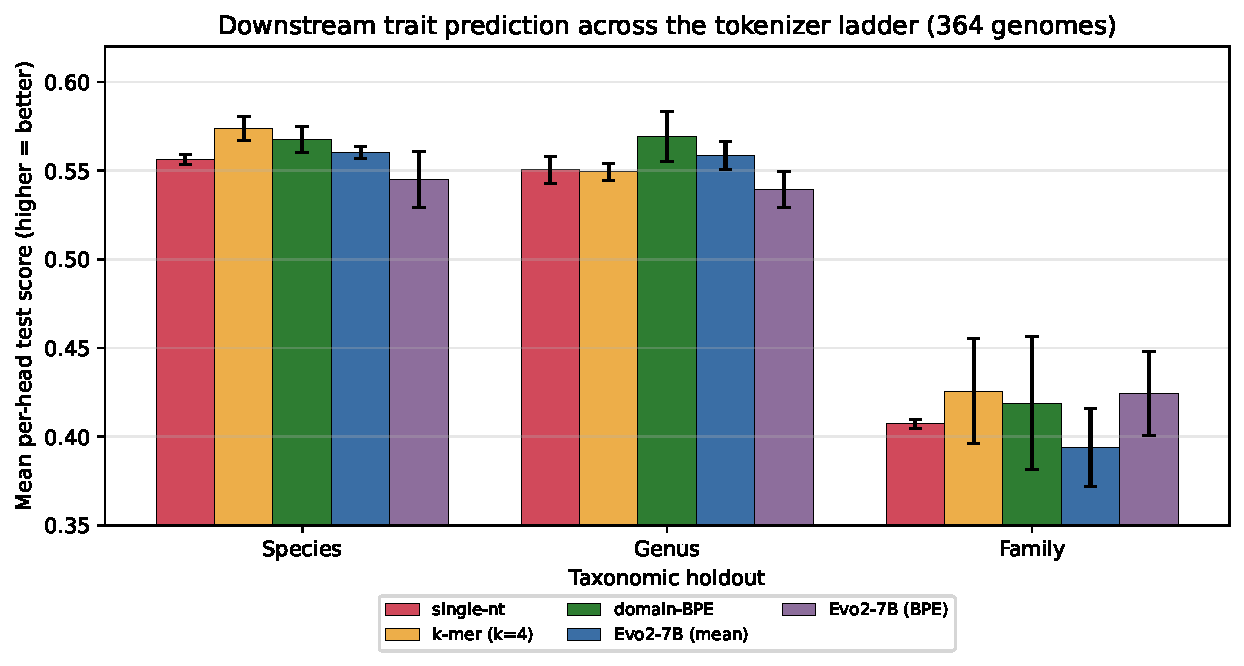
\includegraphics[width=0.86\linewidth]{figs/fig_downstream_bars.pdf}
\caption{Downstream trait prediction across the tokenizer ladder ($364$
genomes, mean per-head score, error bars are std over seeds). Domain BPE is
best or tied-best at every taxonomic holdout and beats the single-nucleotide
control on all three; the $\sim$3\,M-parameter domain-BPE model is competitive
with the $7$B single-nucleotide Evo2 reference.}
\label{fig:microbe-bars}
\end{figure}

\begin{figure}[t]
\centering
\begin{minipage}[t]{0.49\linewidth}
\centering
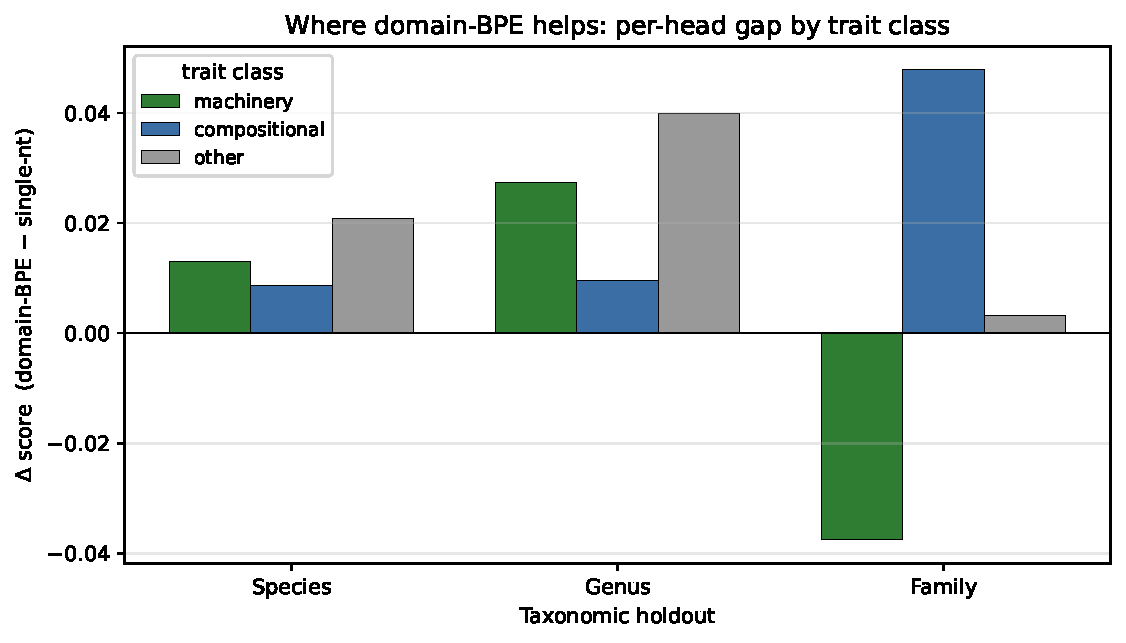
\includegraphics[width=\linewidth]{figs/fig_class_delta.pdf}
\caption{Per-head gap $\Delta$(domain-BPE $-$ single-nt) by trait class and
split. The advantage is consistently positive but small relative to seed noise;
the species machinery/compositional split is where it is most stable.}
\label{fig:microbe-delta}
\end{minipage}\hfill
\begin{minipage}[t]{0.49\linewidth}
\centering
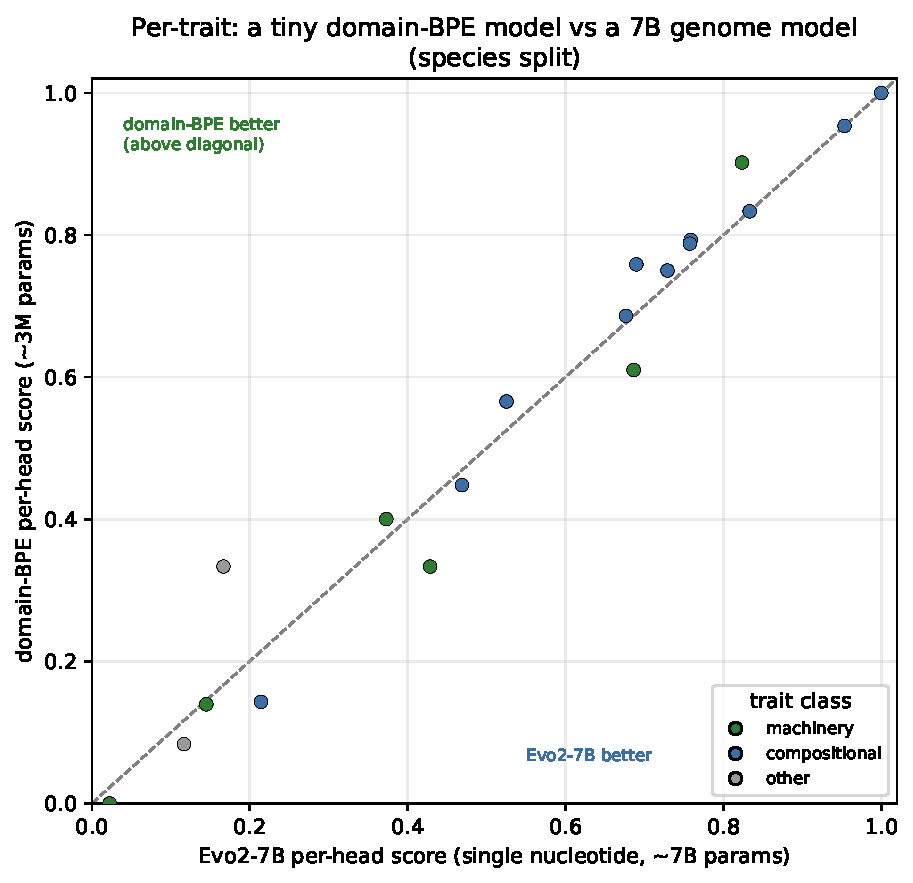
\includegraphics[width=\linewidth]{figs/fig_scatter.pdf}
\caption{Per-trait, species split: a $\sim$3\,M-parameter domain-BPE model
(\(y\)) versus the $7$B single-nucleotide Evo2 (\(x\)). Most heads sit on or
above the diagonal---tokenization buys with $3$M params what scale does not buy
Evo2 with $7$B.}
\label{fig:microbe-scatter}
\end{minipage}
\end{figure}

\paragraph{An honest reading.} We deliberately do not overclaim. The downstream
gaps, while consistently in the predicted direction, are small relative to
seed variance, and only the species split approaches significance; with $364$
genomes the per-class Wilcoxon tests do not cross $p<0.05$. The strong
fixed-$k$-mer baseline (\texttt{kmer\_4}, best at the species split) shows that
much of the immediate benefit here is ``chunks beat single letters,'' with the
sharper ``\emph{learned} chunks beat fixed chunks'' separation remaining within
noise at this scale. This is also consistent with our own \S4.4 caveat: at a
step-matched, CPU-scale budget the held-out bits-per-residue of domain BPE on
this corpus ($1.943$) is not below single-nucleotide ($1.902$), because the
larger BPE softmax is undertrained at fixed steps---yet the representation it
produces is still the more useful one downstream. The load-bearing signals are
therefore qualitative and directional: (i) the Zipfian restoration holds on
real genomic DNA, (ii) domain BPE wins the matched contrast at every taxonomic
level, and (iii) a tiny domain-BPE model is competitive with a $7$B
single-nucleotide foundation model. Microbial traits are largely a function of
gene \emph{content} rather than fine-grained sequence composition, so even a
faint, consistent transfer is the expected footprint of a representational
effect; a compute-matched run over the full BacDive corpus is the natural
confirmation and is left to future work.

% =====================================================================
% PATCH 1 -- Abstract. Append this sentence to the end of the abstract,
% immediately before "We conclude that domain-specific subword tokenization...".
% =====================================================================
%
%   Finally, moving from synthetic probes to a real benchmark, we couple each
%   tokenizer to an external 21-trait microbial-phenotype task over 364 native
%   genomes: domain BPE restores the Zipfian exponent on real genomic DNA
%   ($\alpha\!:\,0.31\!\to\!1.12$), wins the matched single-nucleotide contrast
%   at every taxonomic level, and---at $\sim$3\,M parameters---matches a
%   7-billion-parameter single-nucleotide genome model (Evo2), corroborating the
%   trap where it matters most.

% =====================================================================
% PATCH 2 -- Contributions (\S1). Add as contribution (7).
% =====================================================================
%
%   (7) We move beyond synthetic probes to a \emph{real} downstream benchmark,
%   coupling each tokenizer to an external 21-trait microbial-phenotype task on
%   364 native genomes under strict taxonomic holdouts, and show the trap's
%   predictions transfer: domain BPE restores the Zipfian exponent on real DNA,
%   wins the matched contrast at species/genus/family, and rivals a 7B
%   single-nucleotide gLM (Evo2) at a fraction of the size (\S\ref{sec:microbe}).

% =====================================================================
% PATCH 3 -- Limitations (\S6). Append.
% =====================================================================
%
%   The real-genome benchmark of \S\ref{sec:microbe} removes the
%   reverse-translation and synthetic-task caveats, but at $364$ genomes the
%   downstream gaps, though directionally consistent, are small relative to seed
%   variance and do not reach $p<0.05$ per trait class; a compute-matched run
%   over the full BacDive corpus is required to convert these orderings into
%   significant absolute differences. Microbial traits are also dominated by
%   gene content rather than fine sequence composition, bounding the magnitude
%   of any tokenization effect that can be expected to transfer.
